\section{Введение}

\subsection{Цель работы}

Целью данной лабораторной работы является освоение методики использования измерительного прибора для многократного прямого измерения физической величины, а также выполнение простейшей статистической обработки серии результатов наблюдений при прямых измерениях.

\subsection{Решаемые задачи}

Для достижения поставленной цели необходимо решить следующие задачи:

\begin{enumerate}
    \item Провести многократные прямые измерения периода следования импульсов с помощью электронного частотомера Ч3-32.
    \item Проанализировать временное изменение измеряемой величины и проверить наличие дрейфа.
    \item Построить гистограмму распределения результатов наблюдений и оценить дисперсию.
    \item Рассчитать основные статистические характеристики выборки: среднее арифметическое, среднее квадратическое отклонение, среднюю квадратичную погрешность результата измерения.
    \item Представить окончательный результат измерения в стандартном виде.
\end{enumerate}

\section{Основная часть}

\subsection{Теоретическая часть}

При проведении прямых измерений физической величины истинное значение $X$ остается неизвестным из-за наличия погрешностей. В качестве наилучшего приближения к истинному значению принимается среднее арифметическое результатов отдельных наблюдений:

\begin{equation}
    \bar{x} = \frac{1}{n}\sum_{i=1}^{n} x_i
\end{equation}

Для оценки разброса результатов относительно среднего значения используется среднее квадратическое отклонение (стандартная погрешность отдельного наблюдения):

\begin{equation}
    \sigma = \sqrt{\frac{1}{n-1}\sum_{i=1}^{n} (x_i - \bar{x})^2}
\end{equation}

Средняя квадратичная погрешность результата измерения (погрешность среднего) определяется формулой:

\begin{equation}
    \sigma_{\bar{x}} = \frac{\sigma}{\sqrt{n}}
\end{equation}

Окончательный результат измерения представляется в виде:

\begin{equation}
    x = \bar{x} \pm \Delta x
\end{equation}

где $\Delta x = \sigma_{\bar{x}}$ — оценка средней квадратичной погрешности результата измерения.

\subsection{Эксперимент}

Эксперимент проводился на установке, блок-схема которой представлена на рис.~\ref{fig:scheme}. Измерение периода следования импульсов выполнялось с помощью электронного частотомера Ч3-32. От генератора сигналов Г5-2А на частотомер подавалась последовательность трапецеидальных импульсов.

\begin{figure}[h!]
    \centering
    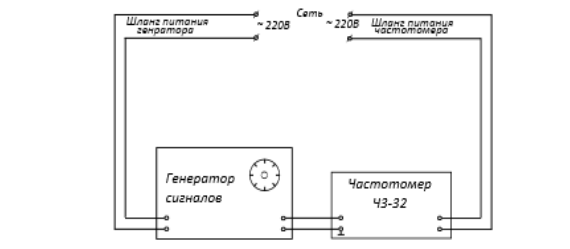
\includegraphics[width=0.8\textwidth]{scheme.png}
    \caption{Блок-схема установки для измерения периода следования импульсов}
    \label{fig:scheme}
\end{figure}

Фотография лабораторной установки представлена на рис.~\ref{fig:setup}.

\begin{figure}[h!]
    \centering
    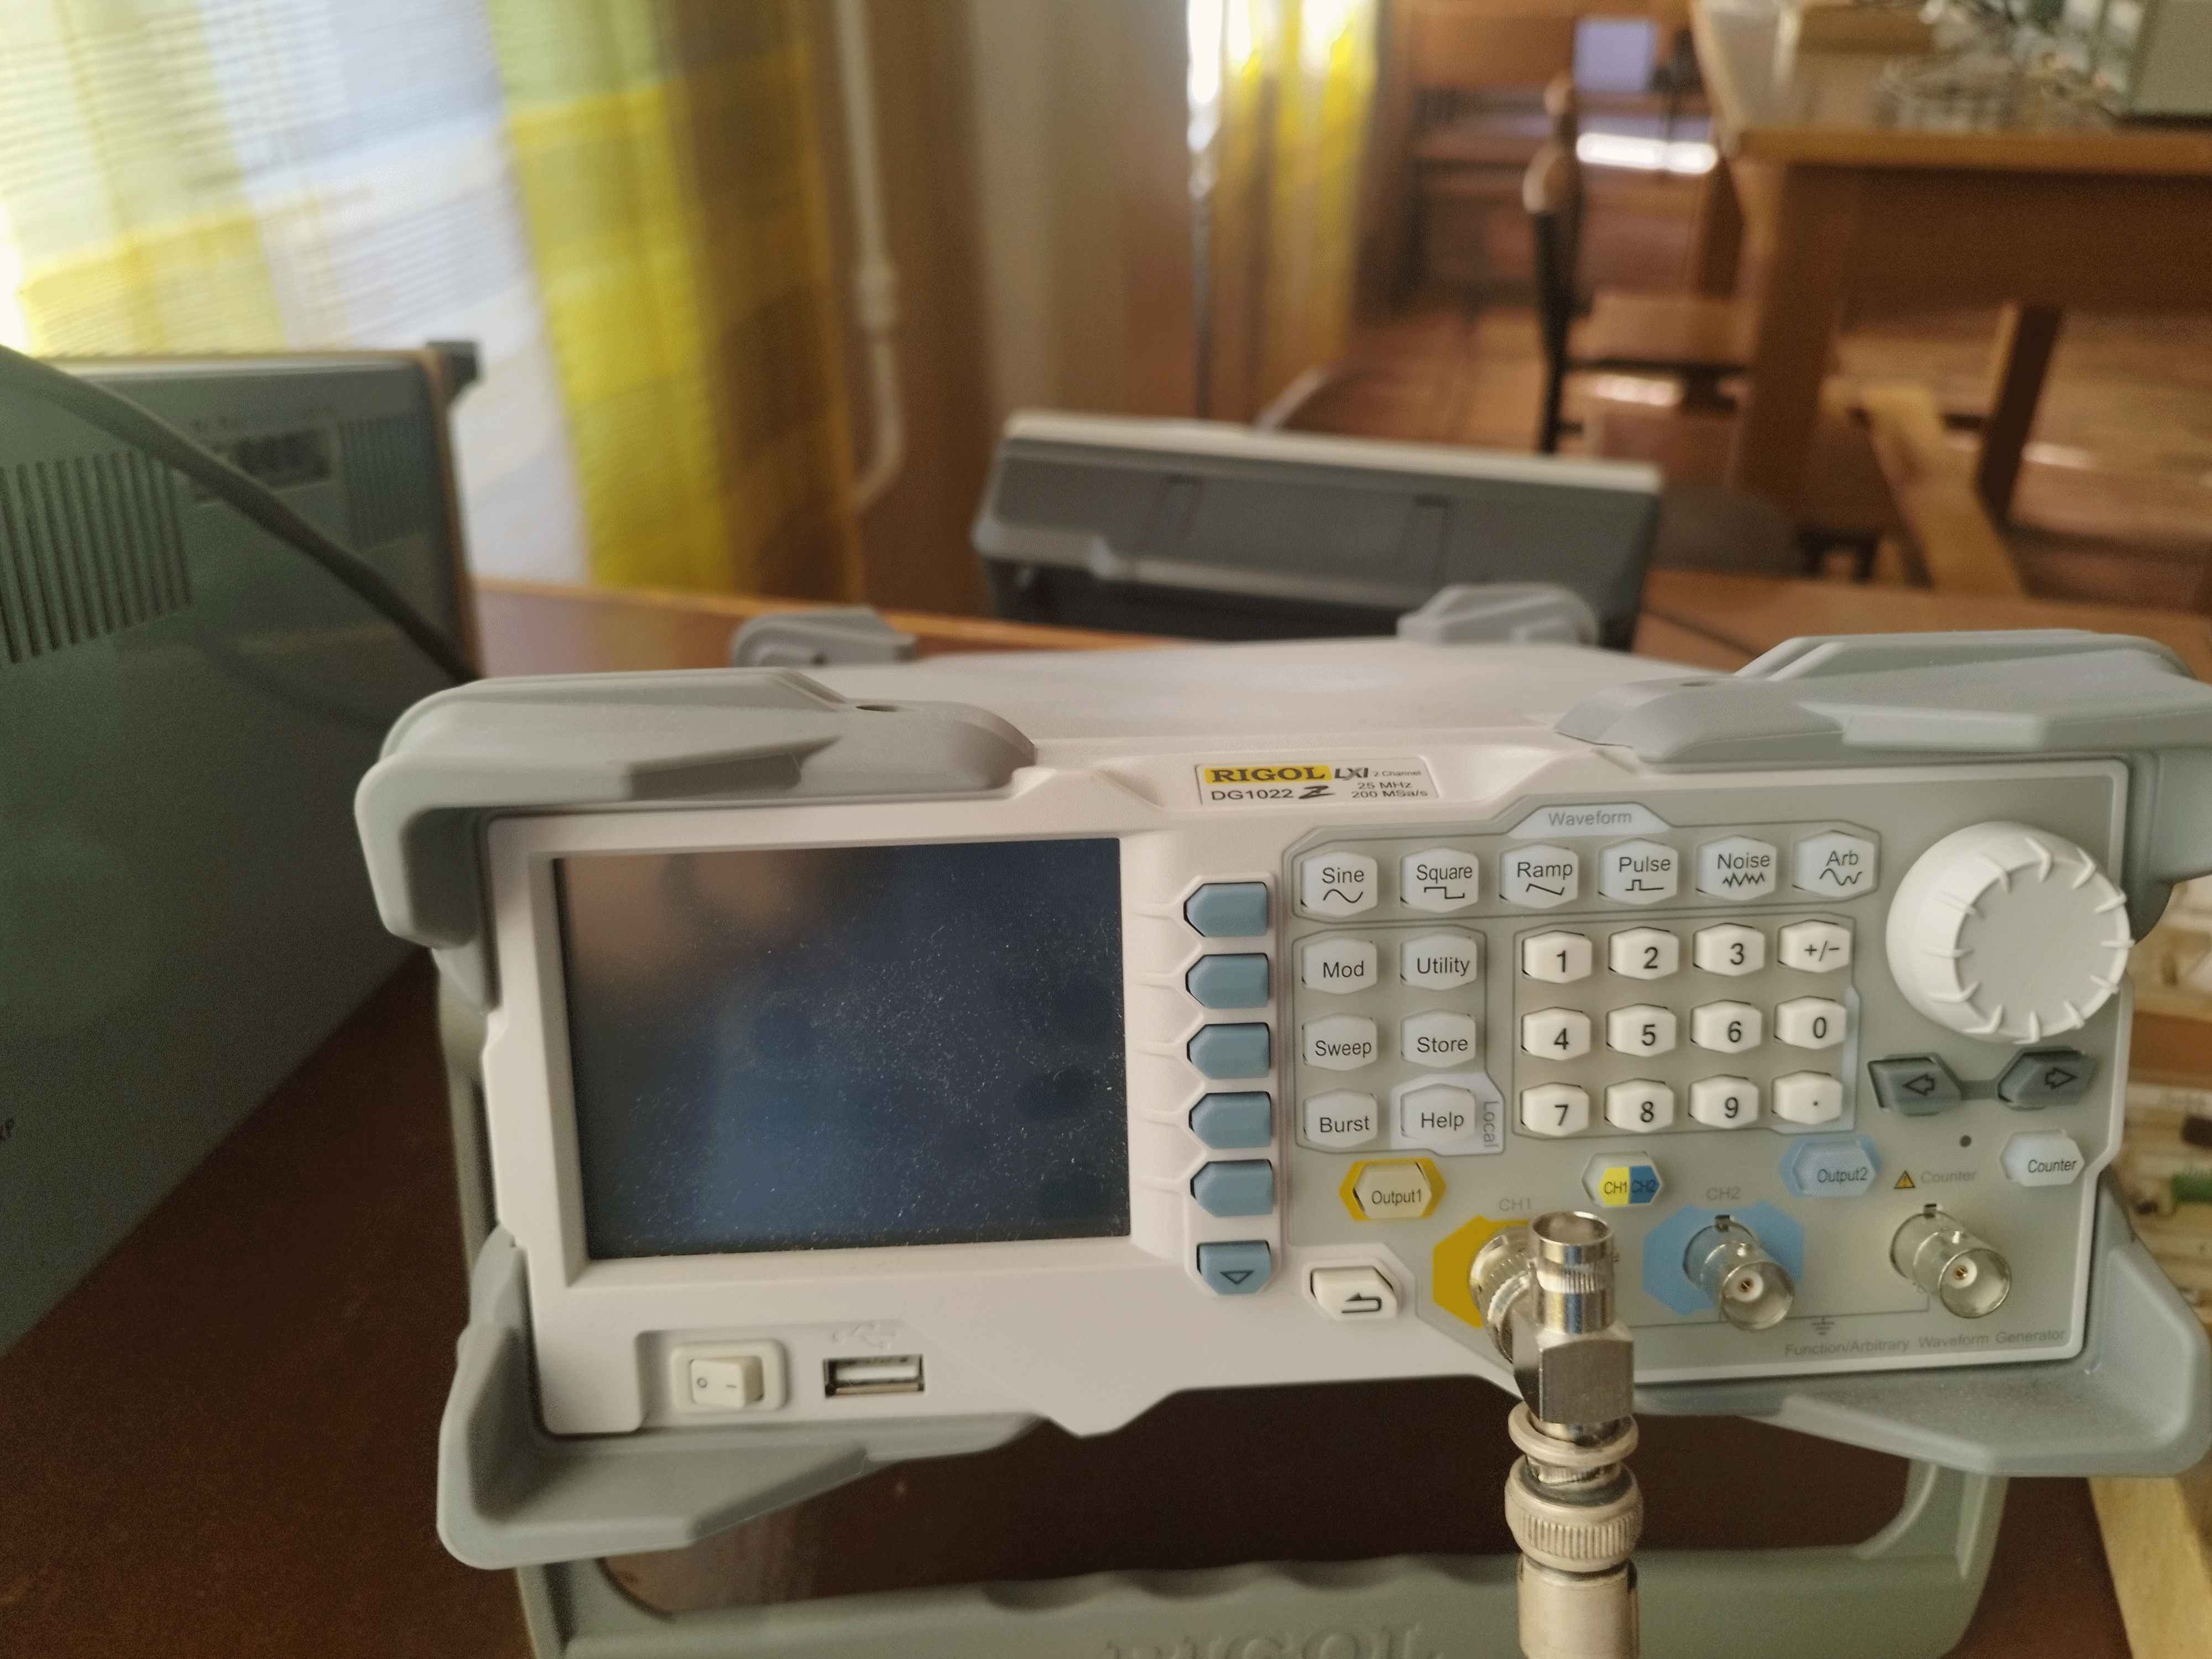
\includegraphics[width=0.8\textwidth]{Device.png}
    \caption{Фотография лабораторной установки}
    \label{fig:setup}
\end{figure}

Порядок выполнения работы:

\begin{enumerate}
    \item Собрана электрическая цепь по блок-схеме, представленной на рис.~\ref{fig:scheme}.
    \item После проверки цепи преподавателем приборы включены в сеть.
    \item Проведены предварительные измерения на грубой шкале прибора (10 измерений).
    \item Выбрана точная шкала прибора и проведена серия из 50 измерений периода следования импульсов.
    \item Результаты измерений занесены в таблицу для последующей обработки.
\end{enumerate}

\subsection{Обработка данных и обсуждение результатов}

Обработка данных выполнена с использованием самостоятельно разработанной программы на языке C++. Визуализация данных осуществлялась с помощью программного обеспечения gnuplot в соответствии с требованиями методических указаний (запрещено использование Microsoft Excel и его аналогов).

\subsubsection{Исходный код}

В листинге~\ref{lst:program} представлена программа для обработки результатов измерений.

\begin{lstlisting}[caption={Программа для обработки результатов измерений}, label={lst:program}]
#include <iostream>
#include <fstream>
#include <vector>
#include <cmath>
#include <iomanip>

int main() {
    std::vector<double> values;
    std::ifstream file("График.txt");
    
    if (!file) {
        std::cerr << "Не удалось открыть файл!" << std::endl;
        return 1;
    }
    
    int number;
    double value;
    while (file >> number >> value) {
        values.push_back(value);
    }
    file.close();
    
    int n = values.size();
    
    // Вычисление среднего
    double sum = 0;
    for (double v : values) sum += v;
    double mean = sum / n;
    
    // Вычисление суммы квадратов отклонений
    double sum_sq_diff = 0;
    for (double v : values) {
        double diff = v - mean;
        sum_sq_diff += diff * diff;
    }
    
    // Вычисление СКО и погрешности среднего
    double sigma = sqrt(sum_sq_diff / (n - 1));
    double sigma_tau = sigma / sqrt(n);
    
    std::cout << std::fixed << std::setprecision(6);
    std::cout << "Результаты обработки:" << std::endl;
    std::cout << "n = " << n << std::endl;
    std::cout << "x = " << mean << " кГц" << std::endl;
    std::cout << "sigma = " << sigma << " кГц" << std::endl;
    std::cout << "delta_x = " << sigma_tau << " кГц" << std::endl;
    
    return 0;
}
\end{lstlisting}

\subsubsection{Анализ временного изменения измеряемой величины}

Для проверки наличия дрейфа результатов измерений построен график зависимости значения от номера измерения (рис.~\ref{fig:drift}).

\begin{figure}[h!]
    \centering
    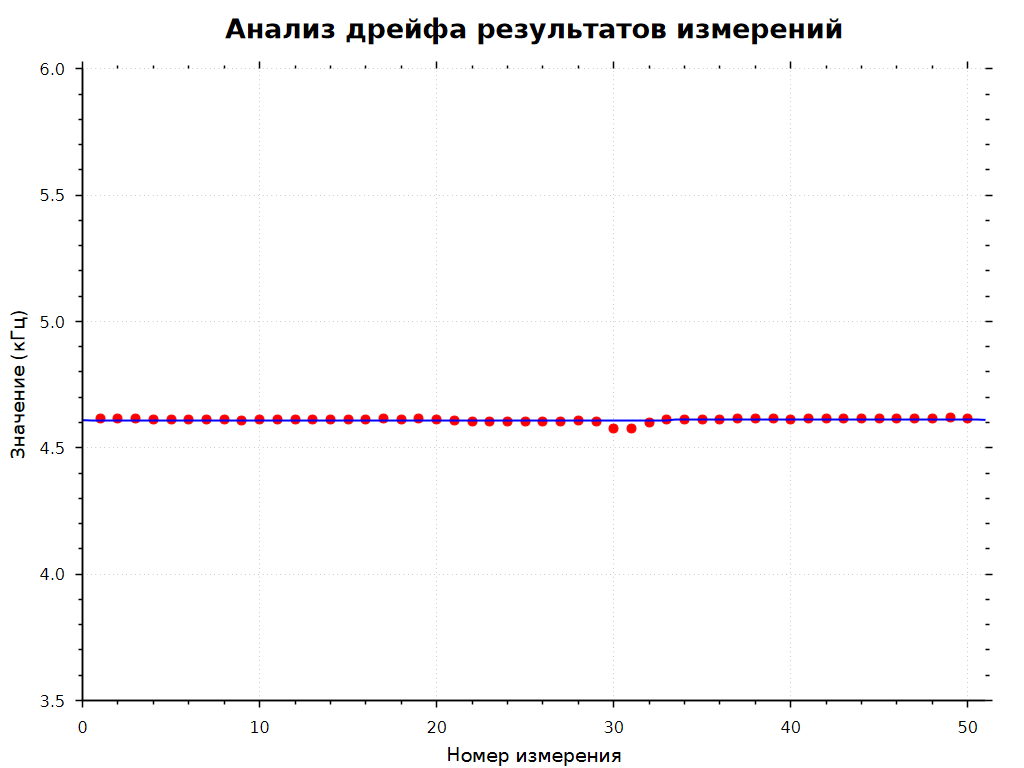
\includegraphics[width=0.9\textwidth]{graph_drift.png}
    \caption{Зависимость результатов наблюдений от времени}
    \label{fig:drift}
\end{figure}

Анализ графика показывает, что значимого дрейфа (монотонного изменения значений с течением времени) не наблюдается. Можно заметить два аномальных измерения (№30 и №31) со значениями 4,576 и 4,578 кГц, которые существенно отличаются от основной массы результатов. За исключением этих выбросов, значения колеблются вокруг среднего без выраженного тренда.

\subsubsection{Нанесение результатов на числовую ось}

На рис.~\ref{fig:individual} представлены результаты отдельных наблюдений, нанесенные на числовую ось с рационально выбранным масштабом.

\begin{figure}[h!]
    \centering
    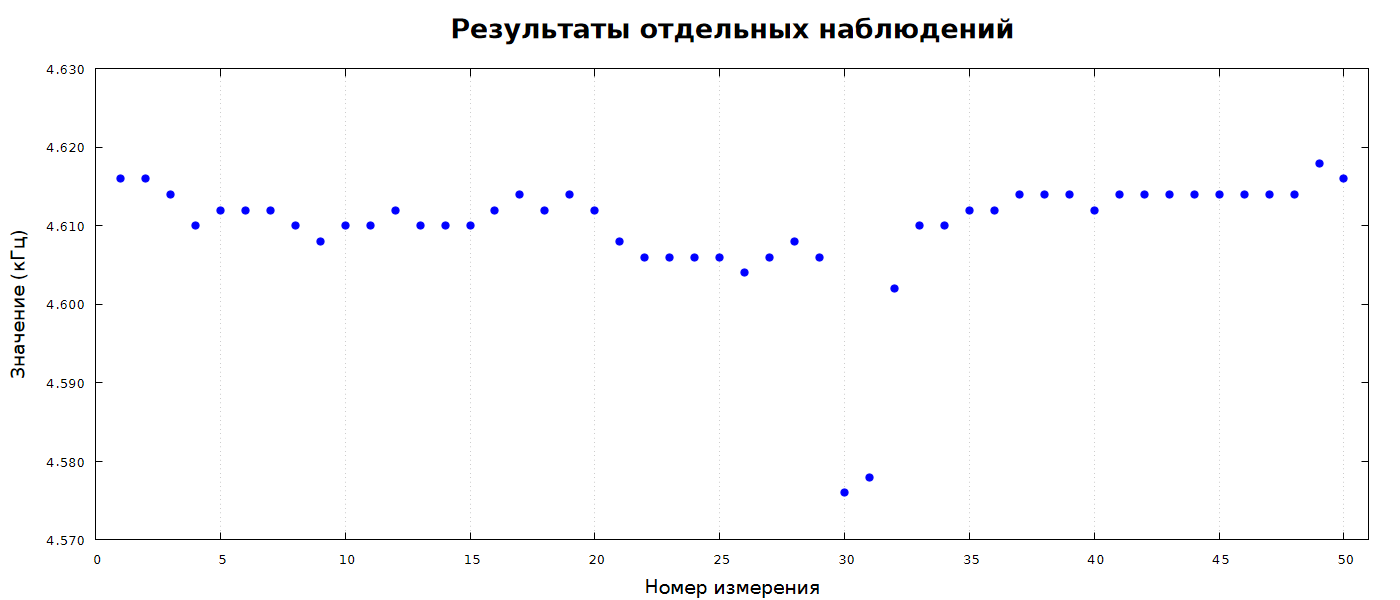
\includegraphics[width=0.9\textwidth]{individual_observations_swapped.png}
    \caption{Результаты отдельных наблюдений на числовой оси}
    \label{fig:individual}
\end{figure}

Диапазон полученных значений:
\begin{itemize}
    \item Минимальное значение: $x_{\text{min}} = 4,576$ кГц
    \item Максимальное значение: $x_{\text{max}} = 4,618$ кГц
    \item Округленные значения: $x_{\text{min}} \approx 4,57$ кГц, $x_{\text{max}} \approx 4,63$ кГц
\end{itemize}

\subsubsection{Построение гистограммы и полигона частот}

Для визуализации распределения результатов измерений построена гистограмма (рис.~\ref{fig:histogram}) и полигон частот (рис.~\ref{fig:polygon}). Весь диапазон от 4,57 до 4,63 кГц разбит на 15 равных интервалов.

\begin{figure}[h!]
    \centering
    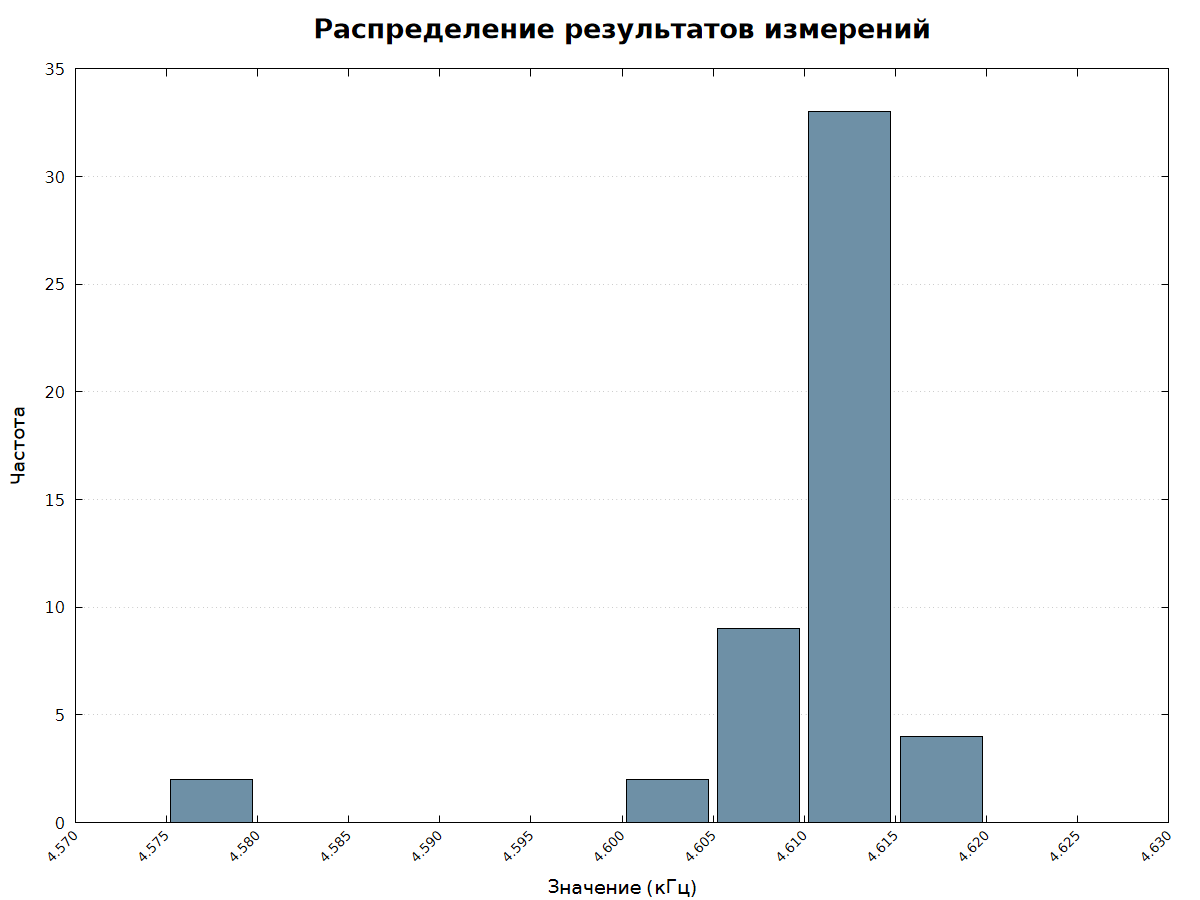
\includegraphics[width=0.8\textwidth]{histogram_simple.png}
    \caption{Гистограмма распределения результатов измерений}
    \label{fig:histogram}
\end{figure}

\begin{figure}[h!]
    \centering
    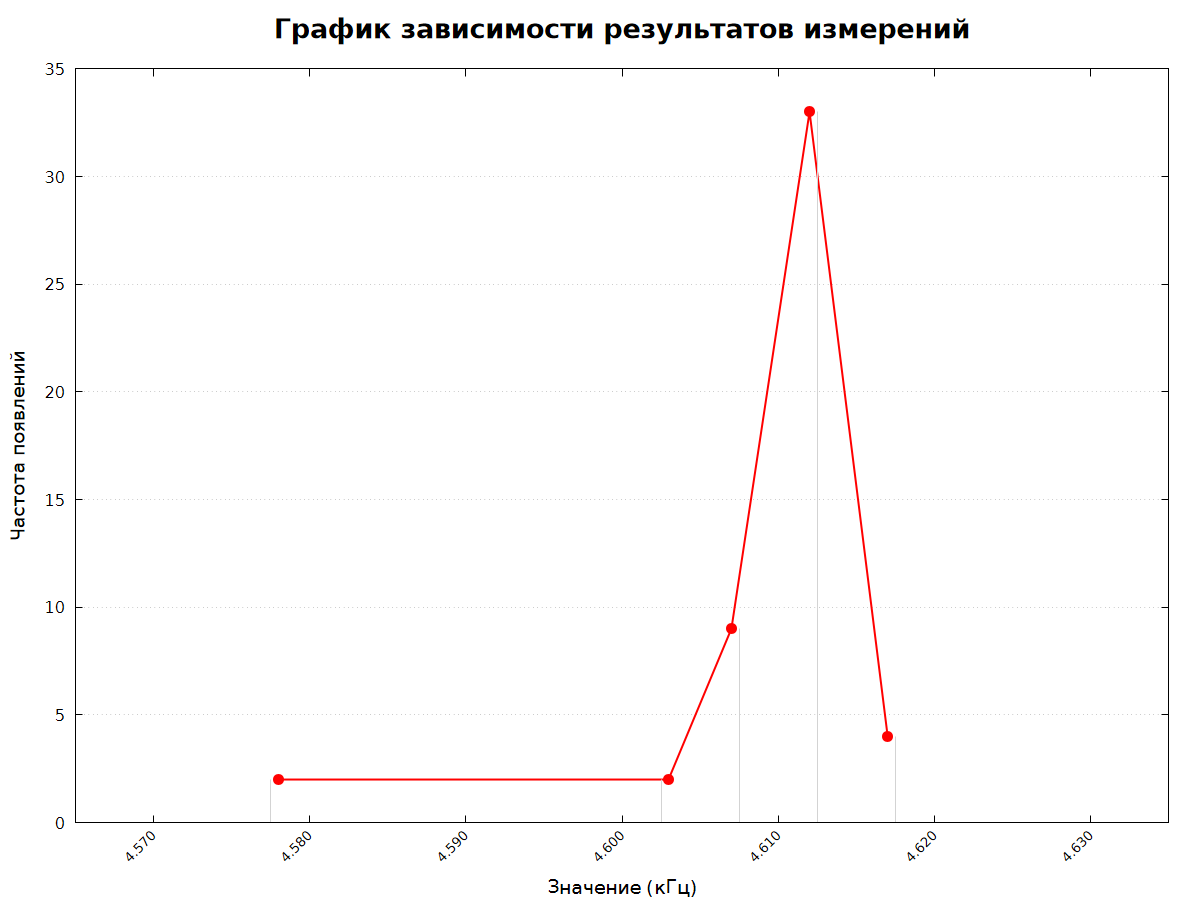
\includegraphics[width=0.8\textwidth]{polygon_frequencies.png}
    \caption{Полигон частот}
    \label{fig:polygon}
\end{figure}

На гистограмме отчетливо видно, что основная масса измерений (более 80\%) сосредоточена в интервале 4,60–4,62 кГц, что указывает на высокую стабильность измерений. Два аномально низких значения (4,576 и 4,578 кГц) проявляются как отдельные пики в левой части гистограммы.

По форме полигона частот можно оценить дисперсию распределения: ширина кривой на уровне примерно 0,6 от максимальной высоты составляет около $2\sigma \approx 0,016$ кГц, откуда $\sigma \approx 0,008$ кГц.

\subsubsection{Таблица результатов наблюдений и отклонений}

В таблице~\ref{tab:measurements} представлены результаты отдельных наблюдений, их отклонения от среднего и квадраты отклонений. Среднее значение вычислено по формуле (1).

\begin{longtable}{|c|c|c|c|}
\caption{Результаты наблюдений и их отклонения от среднего} \label{tab:measurements} \\
\hline
\textbf{№ п/п} & \textbf{$x_i$ (кГц)} & \textbf{$d_i = x_i - \bar{x}$ (кГц)} & \textbf{$d_i^2$ (кГц$^2$)} \\
\hline
\endfirsthead

\hline
\multicolumn{4}{|c|}{\textbf{Продолжение таблицы \ref{tab:measurements}}} \\
\hline
\textbf{№ п/п} & \textbf{$x_i$ (кГц)} & \textbf{$d_i$ (кГц)} & \textbf{$d_i^2$ (кГц$^2$)} \\
\hline
\endhead

\hline
\multicolumn{4}{|r|}{\textit{продолжение на следующей странице}} \\
\endfoot

\hline
\endlastfoot

1 & 4,616 & 0,006 & 0,000036 \\
2 & 4,616 & 0,006 & 0,000036 \\
3 & 4,614 & 0,004 & 0,000016 \\
4 & 4,610 & 0,000 & 0,000000 \\
5 & 4,612 & 0,002 & 0,000004 \\
6 & 4,612 & 0,002 & 0,000004 \\
7 & 4,612 & 0,002 & 0,000004 \\
8 & 4,610 & 0,000 & 0,000000 \\
9 & 4,608 & -0,002 & 0,000004 \\
10 & 4,610 & 0,000 & 0,000000 \\
11 & 4,610 & 0,000 & 0,000000 \\
12 & 4,612 & 0,002 & 0,000004 \\
13 & 4,610 & 0,000 & 0,000000 \\
14 & 4,610 & 0,000 & 0,000000 \\
15 & 4,610 & 0,000 & 0,000000 \\
16 & 4,612 & 0,002 & 0,000004 \\
17 & 4,614 & 0,004 & 0,000016 \\
18 & 4,612 & 0,002 & 0,000004 \\
19 & 4,614 & 0,004 & 0,000016 \\
20 & 4,612 & 0,002 & 0,000004 \\
21 & 4,608 & -0,002 & 0,000004 \\
22 & 4,606 & -0,004 & 0,000016 \\
23 & 4,606 & -0,004 & 0,000016 \\
24 & 4,606 & -0,004 & 0,000016 \\
25 & 4,606 & -0,004 & 0,000016 \\
26 & 4,604 & -0,006 & 0,000036 \\
27 & 4,606 & -0,004 & 0,000016 \\
28 & 4,608 & -0,002 & 0,000004 \\
29 & 4,606 & -0,004 & 0,000016 \\
30 & 4,576 & -0,034 & 0,001156 \\
31 & 4,578 & -0,032 & 0,001024 \\
32 & 4,602 & -0,008 & 0,000064 \\
33 & 4,610 & 0,000 & 0,000000 \\
34 & 4,610 & 0,000 & 0,000000 \\
35 & 4,612 & 0,002 & 0,000004 \\
36 & 4,612 & 0,002 & 0,000004 \\
37 & 4,614 & 0,004 & 0,000016 \\
38 & 4,614 & 0,004 & 0,000016 \\
39 & 4,614 & 0,004 & 0,000016 \\
40 & 4,612 & 0,002 & 0,000004 \\
41 & 4,614 & 0,004 & 0,000016 \\
42 & 4,614 & 0,004 & 0,000016 \\
43 & 4,614 & 0,004 & 0,000016 \\
44 & 4,614 & 0,004 & 0,000016 \\
45 & 4,614 & 0,004 & 0,000016 \\
46 & 4,614 & 0,004 & 0,000016 \\
47 & 4,614 & 0,004 & 0,000016 \\
48 & 4,614 & 0,004 & 0,000016 \\
49 & 4,618 & 0,008 & 0,000064 \\
50 & 4,616 & 0,006 & 0,000036 \\
\hline
\multicolumn{2}{|c|}{\textbf{Сумма}} & \textbf{0,212} & \textbf{0,002952} \\
\hline
\end{longtable}

\subsubsection{Расчет статистических характеристик}

На основе данных таблицы~\ref{tab:measurements} проведены следующие расчеты:

\begin{enumerate}
    \item \textbf{Среднее арифметическое} (по формуле (1)):
    \[
    \bar{x} = \frac{1}{50}\sum_{i=1}^{50} x_i = \frac{230,510}{50} = 4,61020 \text{ кГц}
    \]
    
    \item \textbf{Сумма квадратов отклонений}:
    \[
    \sum_{i=1}^{50} (x_i - \bar{x})^2 = 0,002952 \text{ кГц}^2
    \]
    
    \item \textbf{Среднее квадратическое отклонение (СКО)} (по формуле (2)):
    \[
    \sigma = \sqrt{\frac{1}{n-1}\sum_{i=1}^{n} (x_i - \bar{x})^2} = \sqrt{\frac{0,002952}{49}} = \sqrt{0,00006024} = 0,00776 \text{ кГц}
    \]
    
    \item \textbf{Средняя квадратичная погрешность результата измерения} (по формуле (3)):
    \[
    \sigma_{\bar{x}} = \frac{\sigma}{\sqrt{n}} = \frac{0,00776}{\sqrt{50}} = \frac{0,00776}{7,07107} = 0,00110 \text{ кГц}
    \]
\end{enumerate}

\subsubsection{Сравнение оценок дисперсии}

Оценка дисперсии, полученная по формуле (2): $\sigma = 0,00776$ кГц.

Визуальная оценка по гистограмме (рис.~\ref{fig:histogram}) и полигону частот (рис.~\ref{fig:polygon}) дает значение $\sigma \approx 0,008$ кГц, что хорошо согласуется с расчетным значением.

\subsubsection{Окончательный результат измерения}

В соответствии с формулой (4) результат измерения периода следования импульсов представляется в виде:

\[
f = (4,610 \pm 0,001) \text{ кГц}
\]

Для перевода в период следования импульсов (в миллисекундах) используем соотношение $T = 1/f$:

\[
T = \frac{1}{4,610 \text{ кГц}} = 0,2169 \text{ мс} = (0,217 \pm 0,001) \text{ мс}
\]

Погрешность прибора на точной шкале составляет $\omega = \pm 0,001$ кГц, что сопоставимо с полученной погрешностью результата измерения.

\section{Выводы}

В результате выполнения лабораторной работы были получены следующие результаты:

\begin{enumerate}
    \item Проведены многократные прямые измерения периода следования импульсов (50 наблюдений) с помощью электронного частотомера Ч3-32.
    
    \item Анализ временной зависимости результатов наблюдений (рис.~\ref{fig:drift}) показал отсутствие значимого дрейфа, что свидетельствует о стабильности измеряемой величины в течение эксперимента.
    
    \item Построены гистограмма (рис.~\ref{fig:histogram}) и полигон частот (рис.~\ref{fig:polygon}) распределения результатов измерений. Анализ гистограммы показал, что основная масса измерений (более 80\%) сосредоточена в интервале 4,60–4,62 кГц, что указывает на высокую стабильность измерений. Обнаружены два аномальных измерения (4,576 и 4,578 кГц), которые могут быть классифицированы как промахи.
    
    \item Рассчитаны основные статистические характеристики:
    \begin{itemize}
        \item Среднее значение: $\bar{x} = 4,610$ кГц
        \item Среднее квадратическое отклонение: $\sigma = 0,00776$ кГц
        \item Средняя квадратичная погрешность результата: $\sigma_{\bar{x}} = 0,00110$ кГц
    \end{itemize}
    
    \item Оценка дисперсии по гистограмме ($\sigma \approx 0,008$ кГц) хорошо согласуется с расчетным значением, что подтверждает корректность выполненных вычислений.
    
    \item Окончательный результат измерения представлен в стандартном виде:
    \[
    f = (4,610 \pm 0,001) \text{ кГц} = (0,217 \pm 0,001) \text{ мс}
    \]
\end{enumerate}

Полученная погрешность результата измерения сопоставима с погрешностью используемого прибора, что говорит о корректно проведенных измерениях и отсутствии существенных дополнительных источников погрешностей.


